%!TEX root = CVPR_2018_Nonlinear_3DMM.tex

\Section{Introduction}
\label{sec:intro}
%Importance of 3DMM.
3D Morphable Model (3DMM) is a statistical model of 3D facial shape and texture in a space where there are explicit correspondences~\cite{blanz1999morphable}. 
The morphable model framework provides two key benefits: first, a point-to-point correspondence between the reconstruction and all other models, enabling “morphing”,
and second, modeling underlying transformations between types of faces (male to female, neutral to smile, etc.). 
3DMM has been widely applied in numerous areas, such as computer vision~\cite{blanz1999morphable, yin2017towards}, graphics~\cite{aldrian2013inverse}, human behavioral analysis~\cite{amberg2008expression} and craniofacial surgery~\cite{staal2015describing}.


\begin{figure}[t!]
\centering
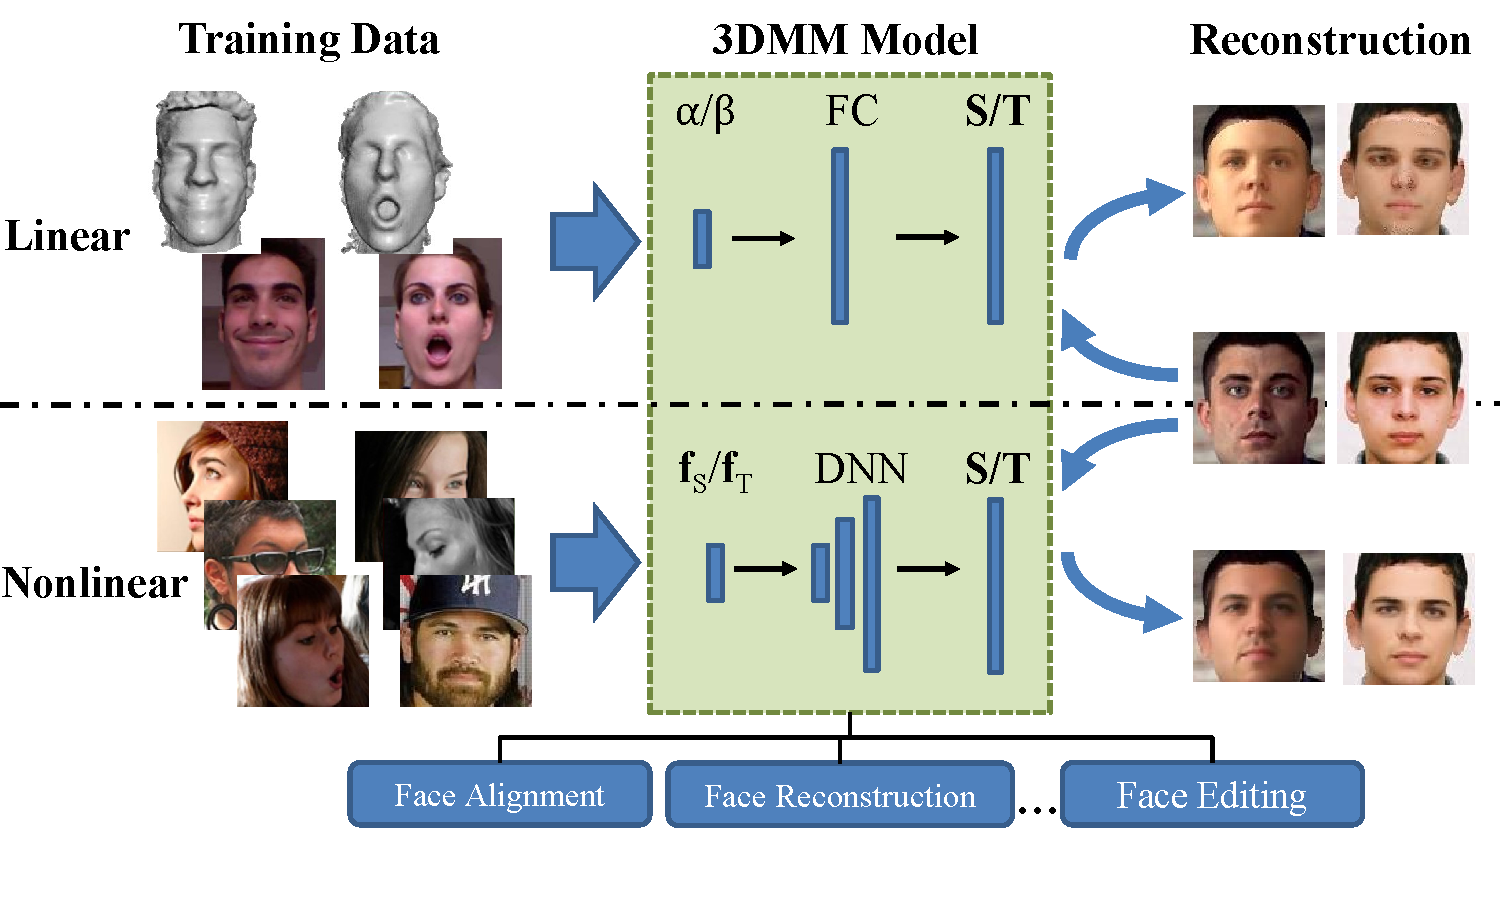
\includegraphics[trim=0 30 12 0, clip, width=\linewidth]{img/Concept.pdf}
\vspace{-4mm}
\caption{\small Conventional 3DMM employs linear bases models for shape/texture, which are trained with 3D face scans and associated controlled 2D images. We propose a nonlinear 3DMM to model shape/texture via deep neural networks~(DNNs). It can be trained from in-the-wild face images without 3D scans, and also better reconstructs the original images due to the inherent nonlinearity.}
\label{fig:concept}
\figvspace 
\end{figure}

% Problem with 3DMM
3DMM is learnt through {\it supervision} by performing dimension reduction, normally Principal Component
Analysis (PCA), on a training set of face images/scans. 
To model highly variable 3D face shapes, a large amount of high-quality 3D face scans is required. 
However, this requirement is expensive to fulfill. 
The first 3DMM~\cite{blanz1999morphable} was built from scans of $200$ subjects with a similar ethnicity/age group. 
They were also captured in well-controlled conditions, with only neutral expressions. 
Hence, it is fragile to large variances in the face identity. 
The widely used Basel Face Model~(BFM)~\cite{paysan20093d} is also built with only $200$ subjects in neutral expressions.  
Lack of expression can be compensated using expression bases from FaceWarehouse~\cite{cao2014facewarehouse} or BD-3FE~\cite{yin20063d}. 
After more than a decade, almost all models use less than $300$ training scans. 
Such a small training set is far from adequate to describe the full variability of human faces~\cite{booth20163d}. 
Only recently, Booth et al.~\cite{booth20163d} spent a significant effort to build 3DMM from scans of ${\sim}10,000$ subjects. % which is still restricted to the public.

Second, the texture model of 3DMM is normally built with a small number of 2D face images {\it co-captured} with 3D scans, under well-controlled conditions.
Therefore, such a model is only learnt to represent the facial texture in similar conditions, rather than in-the-wild environments.
This substantially limits the application scenarios of 3DMM.

Finally, the representation power of 3DMM is limited by not only the size of training set but also its formulation. 
The facial variations are nonlinear in nature. 
E.g., the variations in different facial expressions or poses are nonlinear, which violates the linear assumption of PCA-based models. 
Thus, a PCA model is unable to interpret facial variations well.
% Our approach
Given the barrier of 3DMM in its data, supervision and linear bases, this paper aims to revolutionize the paradigm of learning 3DMM by answering a fundamental question:

%\vspace{0.7mm}
\begin{quote}
{\it Whether and how can we learn a nonlinear 3D Morphable Model of face shape and texture from a set of unconstrained 2D face images, without collecting 3D face scans?}
\end{quote}
%\vspace{0.7mm}

If the answer were yes, this would be in sharp contrast to the conventional 3DMM approach, and remedy all aforementioned limitations.
Fortunately, we have developed approaches that offer positive answers to this question.
%With the recent development of deep neural networks, we view that it is the right time to undertake this new paragram of 3DMM learning.
Therefore, the core of this paper is regarding how to learn this new 3DMM, what is the representation power of the model, and what is the benefit of the model to facial analysis.

%we propose a novel paragram to {\it learn a  non-linear 3DMM model from a large set of unconstrained face images, without collecting 3D face scans}, by leveraging the power of semi-supervised deep neural networks.
%captures variations and structures in complex face data. 
As shown in Fig.~\ref{fig:concept}, starting with an observation that the linear 3DMM formulation is equivalent to a single layer network, using a deep network architecture naturally increases the model capacity. 
Hence, we utilize two network decoders, instead of two PCA spaces, as the shape and texture model components, respectively.
With careful consideration of each component, we design different networks  for shape and texture: the multi-layer perceptron~(MLP) for shape and convolutional neural network~(CNN) for texture.
Each decoder will take a shape or texture representation as input and output the dense 3D face or a face texture.
These two decoders are essentially the nonlinear 3DMM.

Further, we learn the fitting algorithm to our nonlinear 3DMM, which is formulated as a CNN encoder.
The encoder takes a 2D face image as input and generates the shape and texture parameters, from which two decoders estimate the 3D face and texture.
%These representations are decoded by a multi-layer perceptron (shape) or a convolution neural network decoder (texture) to shape and texture respectively. 
The 3D face and texture would {\it perfectly} reconstruct the input face, if the fitting algorithm and 3DMM are well learnt.
Therefore, we design a differentiable rendering layer to generate a reconstructed face by fusing the 3D face, texture, and the camera projection parameters estimated by the encoder. 
Finally, the end-to-end  learning scheme is constructed where the encoder and two decoders are learnt jointly to minimize the difference between the reconstructed face and the input face.
%To make the decoders trainable in end-to-end fashion, we also add the encoder to estimate shape, texture representation together with projection parameters. 
Jointly learning the 3DMM and the model fitting encoder allows us to leverage the large collection of {\it unconstrained} 2D images without relying on 3D scans.
% Implication
We show significantly improved shape and texture representation power over the linear 3DMM. 
Consequently, this also benefits other tasks such as 2D face alignment and 3D reconstruction.


In this paper, we make the following contributions:

1) We learn a \textit{nonlinear} 3DMM model that has greater representation power than its traditional linear counterpart.

2) We jointly learn the model and the model fitting algorithm via \textit{weak supervision}, by leveraging a large collection of 2D images without 3D scans. %The novel spatial-aware texture representation and 
The novel rendering layer enables the end-to-end training.

%that can be efficiently learned or represented by CNN
3) The new 3DMM further improves performance in related tasks: face alignment and face reconstruction.

